\section{论文排版}

\subsection{引用与参考文献}

\begin{frame}[fragile]{引用与参考文献(〇)}
  \begin{description}
    \item[引用] 在正文中出现,用于指出附加信息,十分简短
    \item[参考文献] 在文末出现,用于提供附加信息,按一定顺序罗列
  \end{description}
\end{frame}

\begin{frame}[fragile]{引用与参考文献(一)}
  \begin{enumerate}
    \item 将参考文献条目存储在 |.bib| 文件中
          \begin{itemize}
            \item 每个条目包含文献类型、基本信息以及一个用于引用的键值
            \item 看起来很复杂,但其实不用手动输入
                  \begin{itemize}
                    \item 各种文献管理工具都可以批量导出 |.bib| 格式的条目
                    \item 谷歌学术等文献搜索网站也可以直接复制
                    \item \CJKsout{知网居然连这功能都没有}
                  \end{itemize}
          \end{itemize}
    \item 在文章中添加引用和参考文献
          \begin{itemize}
            \item 导言区
                  \begin{itemize}
                    \item 指定样式:|\bibliographystyle{样式名}|
                    \item 国家标准 GB/T 7714--2015
                          \link{https://github.com/Haixing-Hu/GBT7714-2005-BibTeX-Style/files/153951/GBT.7714-2015.pdf}:
                          \pkg{gbt7714} 宏包
                          %         \item 更多文献、引用样式:\pkg{natbib} 宏包
                  \end{itemize}
            \item 正文区
                  \begin{itemize}
                    \item 标记引用:|\cite{键值}|
                    \item 插入参考文献:|\bibliography{.bib 文件名}|
                  \end{itemize}
          \end{itemize}
  \end{enumerate}
\end{frame}

\begin{frame}[fragile]{引用与参考文献(二)}
  \begin{exampleblock}{示例:\texttt{.bib} 文件}
    \begin{texcode}[gobble=6]
      @incollection{1844_marx_manuscripts,
        author    = {马克思},
        title     = {1844年经济学哲学手稿},
        booktitle = {马克思恩格斯全集},
        publisher = {人民出版社},
        year      = 2002,
        editor    = {马克思 and 恩格斯},
        volume    = 3,
        pages     = {266-280},
        edition   = 2,
        address   = {北京},
        language  = {zh}
      }
    \end{texcode}
  \end{exampleblock}
\end{frame}

\begin{frame}[fragile]{引用与参考文献(三)}
  \begin{exampleblock}{示例:在文章中添加引用和参考文献}
    \begin{texcode}[gobble=6]
      马克思分析了异化劳动的四个方面。\cite{1844_marx_manuscripts}

      \bibliography{reference.bib}
    \end{texcode}
    \vspace{1em}
    \hspace{2em}马克思分析了异化劳动的四个方面。\cite{1844_marx_manuscripts}
    \begin{center}
      \zihao{3} \textsf{参考文献}
    \end{center}
    \renewcommand{\bibsection}{}
    \bibliography{reference.bib}
  \end{exampleblock}
\end{frame}

\begin{frame}[fragile]{引用与参考文献(四)}
  \begin{alertblock}{注意}
    \begin{itemize}
      \item “我都编译了好几次了,怎么还不能正常显示呢?”
            \begin{itemize}
              \item 处理 |.bib| 并非 \TeX{} 引擎本身功能,而要靠 \BibTeX 程序
              \item 通常要先用 \TeX{} 和 \BibTeX 分别编译一遍,再继续用 \TeX{} 编译
              \item 例如:\XeLaTeX $\rightarrow$ \BibTeX $\rightarrow$ \XeLaTeX $\rightarrow$ \XeLaTeX
              \item 再次推荐 \pkg{latexmk}
            \end{itemize}
    \end{itemize}
  \end{alertblock}
  \vspace{-1em}
  \begin{block}{扩展}
    \begin{itemize}
      \item \BibTeX 后端是处理参考文献的传统方法,但功能受限
      \item 更新的方法:\pkg{biber} 后端 + \pkg{biblatex} 宏包
      \item 不过很多模板目前依然采用 \BibTeX,请根据情况选择
    \end{itemize}
  \end{block}
\end{frame}

\subsection{论文模板}

\begin{frame}[fragile]{模板}
  \begin{itemize}
    \item 是什么?
          \begin{itemize}
            \item 设计好的格式框架,可以让用户专注于内容
                  % \item Word 中的样式:「学好 \LaTeX{} 可以更科学地使用 Word」
            \item 以文档类的形式提供,扩展名为 |.cls|
          \end{itemize}
    \item 有哪些?
          \begin{itemize}
            \item 期刊会议:\pkg{revtex}、\pkg{elsarticle}、\pkg{IEEEtran}……
            \item 学位论文:\pkg{thuthesis}、\pkg{ustcthesis}、\hithesis……
          \end{itemize}
    \item 怎么用?
          \begin{itemize}
            \item |\documentclass[模板参数]{模板名}|
            \item 每个模板都可能有独特的用法
                  \begin{itemize}
                    \item \alert{读文档、读文档、读文档}
                    \item \alert{看示例、看示例、看示例}
                  \end{itemize}
          \end{itemize}
    \item 去哪里找?
          \begin{itemize}
            \item 期刊或会议官网
            \item CTAN \link{https://ctan.org} 或 GitHub \link{https://github.com}
            \item 有些模板集成在 TeX 发行版中,但注意确认是否为最新版
          \end{itemize}
  \end{itemize}
\end{frame}

\begin{frame}[fragile]{\hithesis:简介}
  \begin{itemize}
    \item 民间维护的哈工大学位论文 \LaTeX{} 模板
    \item 包括一校三区本科、硕士、博士开题、中期和毕业论文
    \item 生成 PDF 版论文,支持知网查重
    \item 链接:\url{https://github.com/hithesis/hithesis}
    \item 另外,\TeX{} Live 发行版自带本模板,但可能版本滞后
    % \item 未来项目可能迁移至:
    %       \begin{itemize}
    %         \item \url{https://github.com/hithesis/hithesis}
    %       \end{itemize}
  \end{itemize}
\end{frame}

\begin{frame}[fragile]{\hithesis:下载}
  \begin{figure}
    \centering
    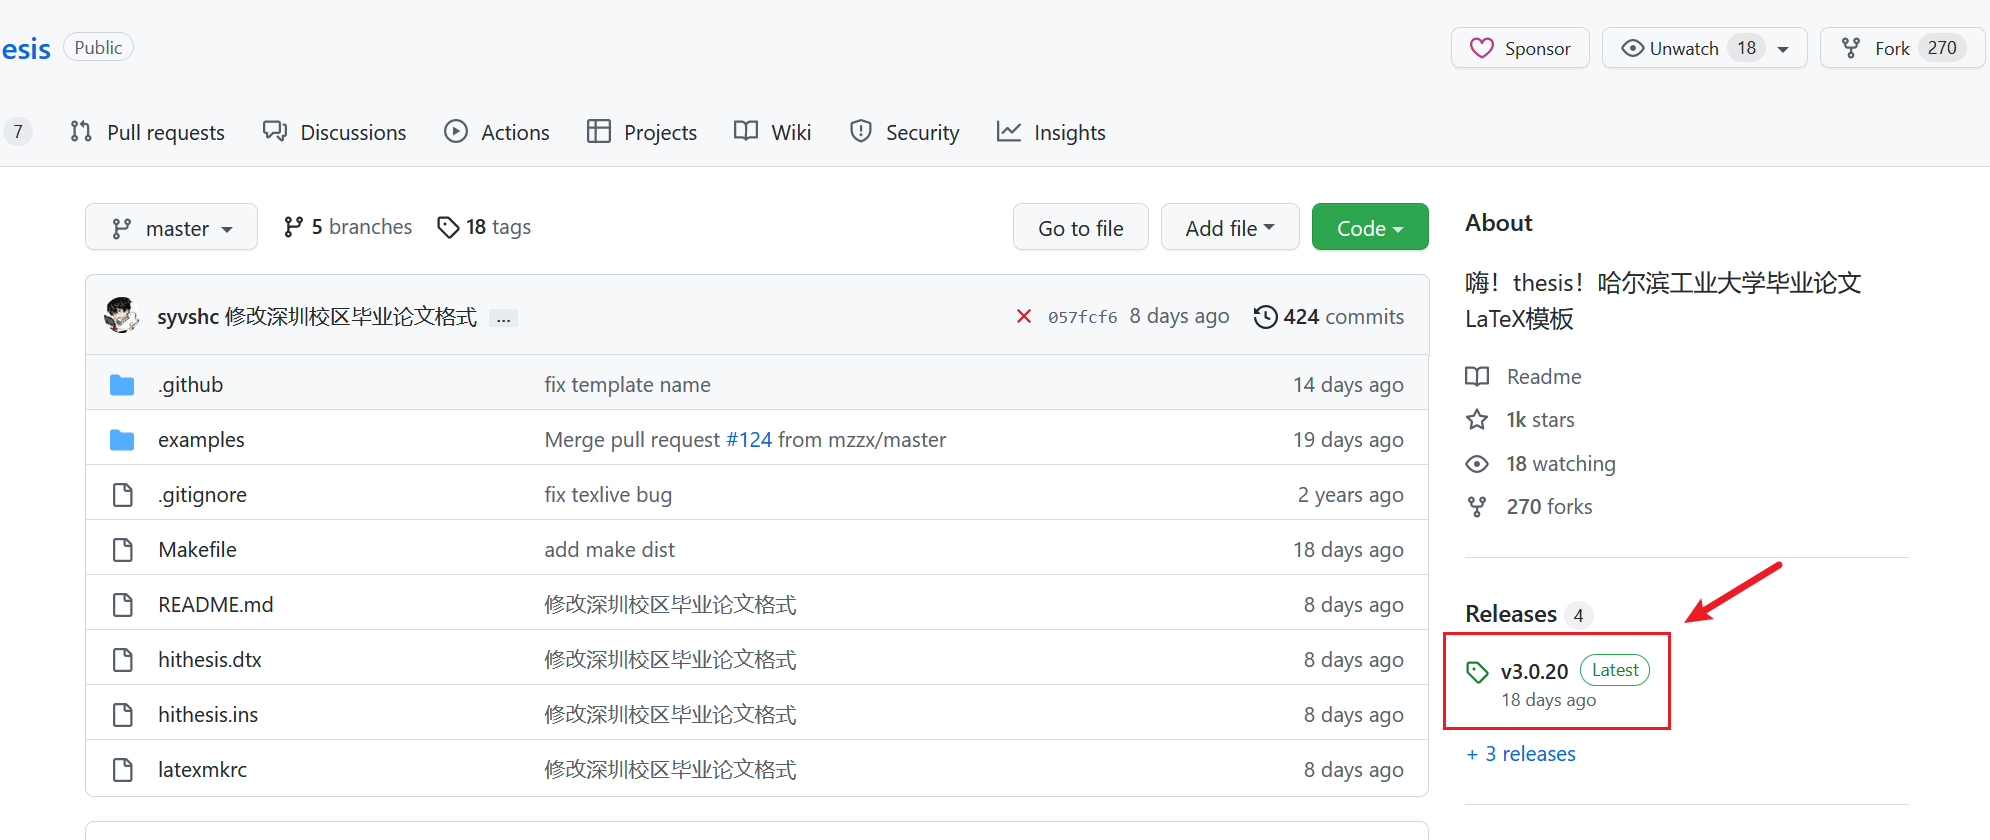
\includegraphics[width=0.8\textwidth]{hithesis_dowload_1.png}
  \end{figure}
  \begin{figure}
    \centering
    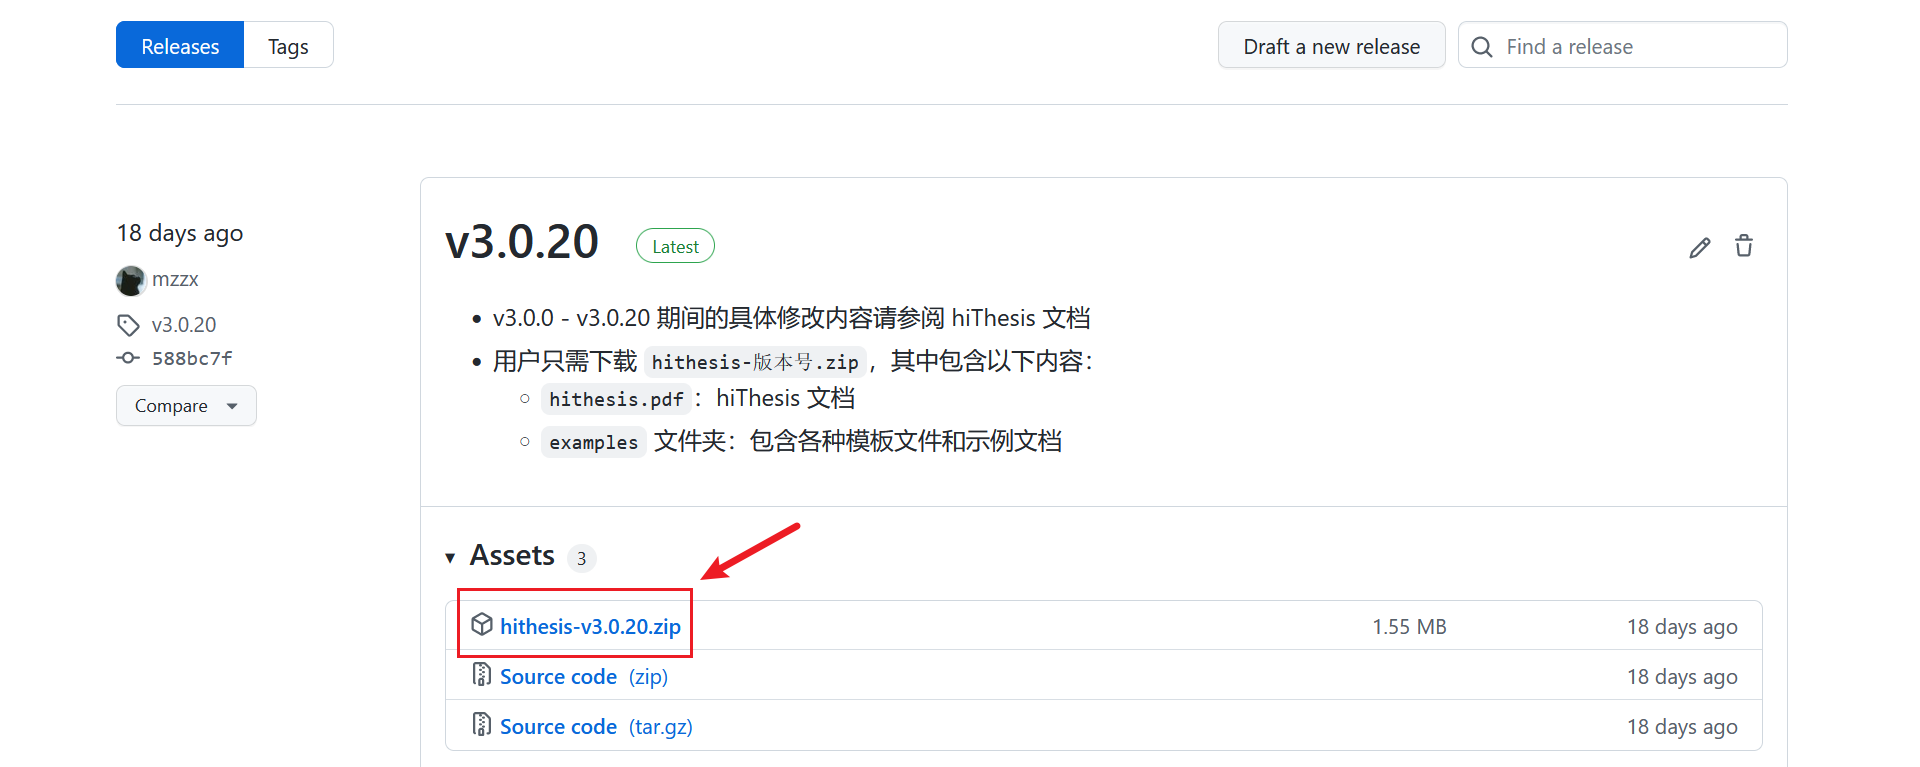
\includegraphics[width=0.8\textwidth]{hithesis_dowload_2.png}
  \end{figure}
\end{frame}

\begin{frame}[fragile]{\hithesis:主目录结构}
  % \dirtree{%
  %   .1 hithesis/.
  %   .2 examples/.
  %   .3 hitart/.
  %   .3 hitbook/.
  %   .2 hithesis.pdf.
  % }
  \hithesis 的主目录结构如下:
  \begin{table}[htbp]
    \begin{tabular}{ll}
      \toprule
      文件名/目录名                           & 描述            \\
      \midrule
      \pkg{example/}                    & 模板示例文件夹       \\
      \pkg{├─ hitart/}                  & 开题和中期报告文件夹    \\
      \pkg{│\phantom{─ }├─ reports/}    & 开题和中期报告文件夹    \\
      \pkg{│\phantom{─ }└─ reportplus/} & 深圳校区博士中期报告文件夹 \\
      \pkg{└─ hitbook/}                 & 毕业论文文件夹       \\
      \pkg{\phantom{├─ }├─ chinese/}    & 中文毕业论文文件夹     \\
      \pkg{\phantom{├─ }└─ english/}    & 英文毕业论文文件夹     \\
      \pkg{hithesis.pdf}                & 用户手册          \\
      \bottomrule
    \end{tabular}
  \end{table}
\end{frame}

% \begin{frame}[fragile]{\hithesis:一个示例的目录结构}
%   \hithesis 示例(以中文毕业论文为例)的目录结构如下:
%   \begin{table}[htbp]
%     \begin{tabular}{ll}
%       \toprule
%       文件名/目录名                           & 描述            \\
%       \midrule
%       \pkg{example/}                    & 模板示例文件夹       \\
%       ├─ \pkg{hitart/}                  & 开题和中期报告文件夹    \\
%       │\phantom{─ }├─ \pkg{reports/}    & 开题和中期报告文件夹    \\
%       │\phantom{─ }└─ \pkg{reportplus/} & 深圳校区博士中期报告文件夹 \\
%       └─ \pkg{hitbook/}                 & 毕业论文文件夹       \\
%       \phantom{│─ }├─ \pkg{chinese/}    & 中文毕业论文文件夹     \\
%       \phantom{│─ }└─ \pkg{english/}    & 英文毕业论文文件夹     \\
%       \pkg{hithesis.pdf}                & 用户手册          \\
%       \bottomrule
%     \end{tabular}
%   \end{table}
% \end{frame}

% \begin{frame}[fragile]{\hithesis:参数}
%   \begin{itemize}
%     \item 常用参数
%           \begin{itemize}
%             \item type\\
%                   doctor/master/bachelor/postdoc\\
%                   (必选)学位:本科/硕士/博士/博士后
%             \item campus\\
%                   shenzhen/weihai/harbin\\
%                   校区:深圳/威海/本部
%             \item fontset\\
%                   windows/mac/ubuntu/fandol/adobe\\
%                   字体:默认会根据系统选择
%           \end{itemize}
%     \item 其他参数请参阅文档
%   \end{itemize}
% \end{frame}

% \begin{frame}[fragile]{\hithesis:开发版}
%   \begin{itemize}
%     \item 常用参数
%           \begin{itemize}
%             \item type\\
%                   doctor/master/bachelor/postdoc\\
%                   (必选)学位:本科/硕士/博士/博士后
%             \item campus\\
%                   shenzhen/weihai/harbin\\
%                   校区:深圳/威海/本部
%             \item fontset\\
%                   windows/mac/ubuntu/fandol/adobe\\
%                   字体:默认会根据系统选择
%           \end{itemize}
%     \item 其他参数请参阅文档
%   \end{itemize}
% \end{frame}
